\documentclass[11pt]{article}

% Change "review" to "final" or remove options to disable line numbers (camera-ready mode)
\usepackage[final]{acl}

% Standard academic typography and encoding
\usepackage{times}
\usepackage{latexsym}
\usepackage[T1,T5]{fontenc}
\usepackage[utf8]{inputenc}

% Aesthetic and spacing enhancements
\usepackage[protrusion=true,expansion=false]{microtype}
\usepackage{inconsolata}

% Mathematics, symbols, and tabular enhancements
\usepackage{amsmath,amssymb}
\usepackage{booktabs}
\usepackage{graphicx}
\usepackage{multirow}
\usepackage{tabularx}
\usepackage{url}
\usepackage{hyperref}

% Author annotation macros for collaborative drafting
\newcommand{\memberone}[1]{\textcolor{blue}{[\textbf{Member 1}: #1]}}
\newcommand{\membertwo}[1]{\textcolor{teal}{[\textbf{Member 2}: #1]}}

\title{Empirical Evaluation of Chunking Strategies for RAG over Structured Technical Documentation}

\author{
  Co-Author One\thanks{~~Equal contribution.} \\
  Department of Computer Science \\
  University / Institution \\
  \texttt{member1@example.edu} \\\And
  Co-Author Two\footnotemark[1] \\
  Department of Computer Science \\
  University / Institution \\
  \texttt{member2@example.edu} \\
}

\begin{document}
\maketitle

\begin{abstract}
\begin{abstract}
Chunking ảnh hưởng trực tiếp đến khả năng truy xuất bằng chứng và chất lượng câu trả lời trong hệ thống \textit{Retrieval-Augmented Generation} (RAG). Nghiên cứu này so sánh ba chiến lược \textit{fixed-size}, \textit{structure-aware} và \textit{prompt-based} trên 384 tài liệu kỹ thuật Angular ở định dạng Markdown. Nhóm đồng thời xây dựng một bộ benchmark gồm 140 câu hỏi gắn với bằng chứng nguồn và đánh giá các chiến lược trong cùng một pipeline được kiểm soát. Kết quả cho thấy \textit{fixed-size} phù hợp hơn khi ưu tiên thứ hạng truy xuất và chất lượng câu trả lời, trong khi \textit{structure-aware} có lợi thế về khả năng thu hồi đầy đủ bằng chứng. \textit{Prompt-based} chưa thể hiện ưu thế nhất quán. Đáng chú ý, khả năng thu hồi bằng chứng tốt hơn không nhất thiết chuyển thành chất lượng câu trả lời cao hơn. Vì vậy, chiến lược chunking cần được lựa chọn theo mục tiêu của hệ thống RAG thay vì dựa trên một chỉ số duy nhất.
\end{abstract}
\end{abstract}

% ==============================================================================
% PHẦN 1 – THÀNH VIÊN 1: CƠ SỞ NGHIÊN CỨU, PHƯƠNG PHÁP VÀ DỮ LIỆU
% ==============================================================================
% ==============================================================================
% 01_introduction.tex
% Phụ trách: Thành viên 1 (Cơ sở nghiên cứu, phương pháp và dữ liệu)
% ==============================================================================
% TODO [Thành viên 1]:
% - Bối cảnh RAG, vai trò trung tâm của chunking trong việc định hình embedding và retrieval.
% - Đặc điểm đặc thù của tài liệu kỹ thuật Markdown (heading hierarchy, fenced code blocks, callouts).
% - Hạn chế của việc coi tài liệu như văn bản phẳng (flat text).
% - Vấn đề nghiên cứu cốt lõi: Bảo toàn cấu trúc tài liệu có thực sự cải thiện hiệu quả RAG hay không?
% - Ba câu hỏi nghiên cứu (RQ1: Retrieval Ranking, RQ2: Evidence Recovery, RQ3: Answer Quality).
% - Ba đóng góp chính của đề tài.
% ==============================================================================

\section{Introduction}
\label{sec:introduction}

Retrieval-Augmented Generation \citep[RAG;][]{lewis2020retrieval} has become the dominant architectural framework for grounding Large Language Models (LLMs) on private, domain-specific, and rapidly updated knowledge bases. 
In software development ecosystems, developer portals and technical documentation serve as the definitive source of truth. 
These technical corpora are almost universally formatted in structured Markdown, featuring rich syntactic elements such as multi-tiered heading hierarchies (\texttt{\#}, \texttt{\#\#}, \texttt{\#\#\#}), fenced code blocks with explicit language tags, structured tables, and informational callout admonitions.

At the core of every RAG system lies document chunking---the process of partitioning continuous source texts into discrete, indexed units. 
Despite the sophisticated structure of technical Markdown, prevailing industrial pipelines treat documents as flat, unstructured text streams, segmenting them via arbitrary character or token counts. 
This flat text assumption introduces critical syntactic and semantic failure modes:
\begin{itemize}
    \item \textbf{Syntactic Bisection:} Arbitrary windowing indiscriminately severs code blocks, leaving dangling delimiters or splitting function calls away from their type definitions and import statements.
    \item \textbf{Contextual Disconnect:} Subsections and explanatory paragraphs lose their parent structural ancestry, producing embeddings that are semantically ungrounded.
    \item \textbf{Diluted Evidence Recovery:} When evidence for a technical query spans multiple related sub-blocks, naive splitting scatters these fragments across unrelated chunks.
\end{itemize}

\begin{figure*}[t]
    \centering
    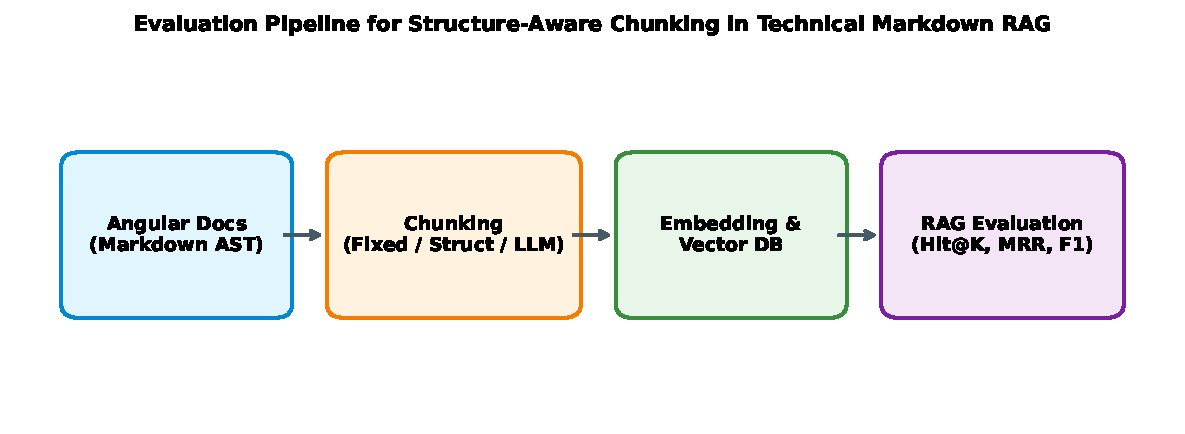
\includegraphics[width=0.92\textwidth]{figures/pipeline_placeholder.pdf}
    \caption{Overview of the controlled evaluation framework: 384 Angular technical Markdown documents are segmented under three chunking strategies (Fixed-size, Structure-aware, Prompt-based), indexed into dense embeddings, and evaluated under identical retrieval and context budgets against 140 expert-curated QA pairs.}
    \label{fig:pipeline_overview}
\end{figure*}

\subsection{Research Problem and Questions}
These pervasive limitations raise a fundamental empirical question: \textit{Does explicitly preserving document structure during chunking genuinely improve end-to-end RAG performance, or does it introduce new structural trade-offs?} 
To rigorously answer this question, we formulate three targeted Research Questions (RQs):
\begin{itemize}
    \item \textbf{RQ1 (Retrieval Ranking):} How does structure-aware chunking compare to fixed-size sliding windows and prompt-based chunking in early-stage retrieval ranking (Hit@$K$, MRR)?
    \item \textbf{RQ2 (Evidence Recovery):} To what extent does preserving heading hierarchy and atomic block boundaries improve the retrieval coverage of complete gold evidence spans (Evidence Coverage, All-Evidence-Retrieved Rate)?
    \item \textbf{RQ3 (Answer Generation Quality):} How do the resulting chunk granularities and retrieval contexts impact downstream response fidelity (Token Precision, Token Recall, and Token F1)?
\end{itemize}

\subsection{Main Contributions}
This research delivers three core contributions to the study of RAG on technical corpora:
\begin{enumerate}
    \item \textbf{A Standardized Technical Documentation Benchmark:} We build and release an expert-validated benchmark based on 384 Angular Markdown documents, containing 140 curated QA pairs stratified across three difficulty levels (60 easy, 40 medium, 40 hard) with 233 granular evidence spans completely decoupled from chunk boundaries.
    \item \textbf{Controlled Comparative Framework:} We systematically benchmark three representative chunking paradigms---Fixed-size, Structure-aware (AST), and Prompt-based (LLM with local validation)---under identical embedding, retrieval budget (2,048 tokens), and context budget (4,096 tokens) constraints.
    \item \textbf{Empirical Trade-off Characterization:} We identify and explain key trade-offs between early-rank retrieval precision and broad evidence recall, proving that no single chunking strategy dominates across all RAG objectives and providing actionable architectural guidelines for practitioners.
\end{enumerate}

% 02_related_work.tex
% Phụ trách: Thành viên 1
% ==============================================================================

\section{Related Work}
\label{sec:related-work}

\subsection{Chunking Strategies}

Chunking quyết định đơn vị văn bản được embedding và truy xuất trong hệ thống RAG \citep{lewis-etal-2020-rag}. Các phương pháp hiện có có thể được phân thành năm nhóm chính.

\paragraph{Fixed-size chunking.}
Phương pháp này chia văn bản thành các cửa sổ có số token hoặc ký tự cố định, thường kèm overlap để giảm mất thông tin tại ranh giới. Fixed-size dễ triển khai và kiểm soát chi phí, nhưng không xét đến cấu trúc hoặc tính liên kết ngữ nghĩa của nội dung \citep{qu-etal-2025-semantic}.

\paragraph{Sentence- and paragraph-based chunking.}
Nhóm phương pháp này sử dụng câu hoặc đoạn văn làm ranh giới tự nhiên. Cách tiếp cận này hạn chế việc cắt giữa câu nhưng có thể tạo ra các chunk có kích thước không đồng đều hoặc tách rời những phần nội dung phụ thuộc lẫn nhau \citep{qu-etal-2025-semantic}.

\paragraph{Semantic chunking.}
Semantic chunking xác định ranh giới dựa trên mức độ tương đồng embedding giữa các câu liên tiếp. Mục tiêu là duy trì tính liên kết ngữ nghĩa, nhưng phương pháp này làm tăng chi phí xử lý và chưa cho thấy lợi ích nhất quán so với fixed-size chunking \citep{qu-etal-2025-semantic}.

\paragraph{Structure-aware chunking.}
Structure-aware chunking khai thác heading hierarchy, paragraph, list, table, code block hoặc abstract syntax tree (AST). Các thành phần có quan hệ được tổ chức theo cấu trúc phân cấp nhằm bảo toàn ngữ cảnh của tài liệu \citep{jain-etal-2025-autochunker}.

\paragraph{LLM-assisted chunking.}
LLM-assisted hoặc prompt-based chunking sử dụng language model để xác định các đơn vị nội dung và đề xuất ranh giới linh hoạt. Các phương pháp như PIC và AutoChunker cho thấy khả năng kết hợp tín hiệu ngữ nghĩa với cấu trúc tài liệu, nhưng yêu cầu thêm chi phí suy luận và cơ chế kiểm soát đầu ra \citep{wang-etal-2025-document,jain-etal-2025-autochunker}.

\subsection{Evaluation of RAG Systems}

Đánh giá RAG thường được thực hiện ở nhiều cấp độ \citep{yu-etal-2024-rag-evaluation}. Ở cấp retrieval, Hit@\(K\), Recall@\(K\) và Mean Reciprocal Rank (MRR) đo khả năng truy xuất và xếp hạng nguồn liên quan. Ở cấp evidence, Evidence Coverage và All-Evidence-Retrieved Rate phản ánh mức độ thu hồi các bằng chứng cần thiết. Ở cấp câu trả lời, các chỉ số như Token F1, BLEU và ROUGE đo mức độ tương đồng với đáp án tham chiếu; human evaluation có thể bổ sung đánh giá về tính chính xác và đầy đủ. Việc phân biệt ba cấp độ là cần thiết vì cải thiện retrieval hoặc evidence recovery không nhất thiết dẫn đến chất lượng câu trả lời cao hơn \citep{qu-etal-2025-semantic}.

\subsection{Research Gap}

Các nghiên cứu gần đây đã so sánh fixed-size với semantic chunking hoặc đề xuất phương pháp phân đoạn mới \citep{qu-etal-2025-semantic,wang-etal-2025-document}. Tuy nhiên, tác động của việc bảo toàn cấu trúc tài liệu đến retrieval ranking, evidence recovery và answer quality vẫn chưa được đánh giá đầy đủ trong cùng một thiết lập trên tài liệu kỹ thuật có cấu trúc. Nghiên cứu này giải quyết khoảng trống đó bằng cách so sánh fixed-size, structure-aware và prompt-based chunking trong một pipeline được kiểm soát, đồng thời đánh giá riêng biệt cả ba cấp độ.
% ==============================================================================
% 03_dataset.tex
% Phụ trách: Thành viên 1 (Cơ sở nghiên cứu, phương pháp và dữ liệu)
% ==============================================================================
% TODO [Thành viên 1]:
% - Mô tả corpus 384 tài liệu Angular Markdown, cấu trúc tài liệu và tiền xử lý.
% - Quá trình dùng ChatGPT hỗ trợ tạo QA ban đầu.
% - Quá trình 3 kỹ sư phần mềm review tuần tự (sequential expert review).
% - Cấu trúc mỗi QA record & NGUYÊN TẮC QUAN TRỌNG: không gắn ground truth với chunk ID
%   (để đảm bảo tính trung lập khi đánh giá các chiến lược chunking khác nhau).
% - Bảng thống kê chi tiết: 140 câu hỏi, 233 evidence items, 60 easy, 40 medium, 40 hard.
% - Phân bố phạm vi: single-section, cross-section, cross-document.
% - Giải thích tiêu chí thiết kế độ khó và các nhóm câu hỏi trong benchmark.
% ==============================================================================

% 03_dataset.tex
% Phụ trách: Thành viên 1
% ==============================================================================

\section{Corpus and QA Benchmark}
\label{sec:dataset}

\subsection{Technical Document Corpus}

Corpus gồm 384 tài liệu kỹ thuật Angular ở định dạng Markdown. Các tài liệu có cấu trúc phân cấp thông qua heading và chứa nhiều loại block như paragraph, list, table, code block và callout. Đặc điểm này cho phép đánh giá ảnh hưởng của việc bảo toàn cấu trúc tài liệu trong quá trình chunking.

Trong bước tiền xử lý, mỗi tài liệu được phân tích thành chuỗi block theo thứ tự xuất hiện trong nguồn. Đối với mỗi block, hệ thống lưu loại nội dung, văn bản gốc và đường dẫn heading tương ứng. Nội dung không được tóm tắt hoặc viết lại nhằm bảo toàn bằng chứng nguồn cho quá trình đánh giá.

\subsection{QA Benchmark Construction}

Do chưa có benchmark phù hợp trực tiếp với corpus và mục tiêu nghiên cứu, nhóm xây dựng một bộ câu hỏi--trả lời có gắn bằng chứng nguồn. ChatGPT được sử dụng để hỗ trợ tạo câu hỏi ứng viên, đáp án tham chiếu và vùng bằng chứng ban đầu. Các đầu ra này chỉ được xem là bản nháp và không được đưa trực tiếp vào benchmark cuối cùng.

Mỗi mẫu sau đó trải qua \textit{sequential expert review} bởi ba kỹ sư phần mềm có từ bốn đến năm năm kinh nghiệm. Các chuyên gia lần lượt kiểm tra và chỉnh sửa câu hỏi, đáp án, loại câu hỏi, kiểu suy luận, độ khó và bằng chứng nguồn. Một mẫu chỉ được chấp nhận khi có thể trả lời đầy đủ từ corpus và không phụ thuộc vào kiến thức bên ngoài.

\subsection{Data Structure and Chunk-Neutral Ground Truth}

Mỗi QA record gồm các trường chính sau:

\begin{itemize}
    \item \texttt{question\_id}: mã định danh của câu hỏi;
    \item \texttt{question}: nội dung câu hỏi;
    \item \texttt{reference\_answer}: đáp án tham chiếu;
    \item \texttt{difficulty}: mức độ easy, medium hoặc hard;
    \item \texttt{question\_type}: loại câu hỏi;
    \item \texttt{reasoning\_type}: kiểu suy luận cần thiết;
    \item \texttt{evidence}: danh sách các evidence item.
\end{itemize}

Mỗi evidence item lưu mã bằng chứng, mã tài liệu, đường dẫn section và các câu chứa bằng chứng. Ground truth được liên kết với nội dung tài liệu gốc thay vì chunk được tạo bởi một phương pháp cụ thể. Benchmark không lưu \texttt{chunk\_id}, \texttt{relevant\_chunk\_id} hoặc nhãn phụ thuộc vào chiến lược chunking. Nguyên tắc này cho phép cùng một ground truth được sử dụng công bằng cho fixed-size, structure-aware và prompt-based chunking.

\subsection{Benchmark Statistics}

Benchmark cuối cùng gồm 140 câu hỏi và 233 evidence items. Phân bố theo độ khó được trình bày trong Bảng~\ref{tab:difficulty-distribution}.

\begin{table}[t]
\centering
\small
\begin{tabular}{lrr}
\toprule
\textbf{Độ khó} & \textbf{Số câu} & \textbf{Tỷ lệ} \\
\midrule
Easy   & 60  & 42.9\% \\
Medium & 40  & 28.6\% \\
Hard   & 40  & 28.6\% \\
\midrule
Tổng   & 140 & 100.0\% \\
\bottomrule
\end{tabular}
\caption{Phân bố câu hỏi theo độ khó.}
\label{tab:difficulty-distribution}
\end{table}

Các câu hỏi còn được phân loại theo phạm vi bằng chứng. \textit{Single-section} sử dụng bằng chứng trong một section; \textit{cross-section} kết hợp nhiều section trong cùng tài liệu; và \textit{cross-document} yêu cầu bằng chứng từ nhiều tài liệu. Phân bố tương ứng được trình bày trong Bảng~\ref{tab:evidence-scope}.

\begin{table}[t]
\centering
\small
\begin{tabular}{lr}
\toprule
\textbf{Phạm vi bằng chứng} & \textbf{Số câu} \\
\midrule
Single-section & 50 \\
Cross-section  & 60 \\
Cross-document & 30 \\
\midrule
Tổng           & 140 \\
\bottomrule
\end{tabular}
\caption{Phân bố câu hỏi theo phạm vi bằng chứng.}
\label{tab:evidence-scope}
\end{table}

\subsection{Difficulty Design}

Độ khó được xác định dựa trên số vùng bằng chứng, độ phức tạp suy luận, mức độ phụ thuộc giữa các phần tài liệu và phạm vi thông tin cần bao phủ. Tất cả câu hỏi đều phải có đủ bằng chứng trong corpus; nhãn hard không biểu thị câu hỏi mơ hồ hoặc thiếu thông tin.

Câu hỏi easy chủ yếu thuộc nhóm fact hoặc definition và dựa trên một vùng bằng chứng cục bộ. Câu hỏi medium yêu cầu kết hợp hai evidence items, thường thuộc các nhóm comparison, procedure, cause--effect hoặc multi-fact synthesis. Trong 40 câu medium, 27 câu có hai evidence items trong cùng một section và 13 câu sử dụng bằng chứng từ nhiều section. Câu hỏi hard kết hợp từ hai đến ba vùng bằng chứng và có thể yêu cầu tổng hợp, phân tích trade-off, theo dõi thay đổi trạng thái hoặc đối chiếu thông tin phân tán.
% 04_chunking_strategies.tex
% Phụ trách: Thành viên 1
% ==============================================================================

\section{Chunking Strategies}
\label{sec:chunking-strategies}

Nghiên cứu so sánh ba chiến lược chunking trên cùng corpus. Mỗi chiến lược tạo một tập chunk độc lập, trong đó kích thước mỗi chunk không vượt quá 512 token.

\subsection{Fixed-size Chunking}

Fixed-size tuyến tính hóa tài liệu theo thứ tự nguồn và chia văn bản thành các cửa sổ 512 token, với 64 token overlap giữa hai cửa sổ liên tiếp. Phương pháp không sử dụng heading hoặc cấu trúc phân cấp khi xác định ranh giới. Kết quả tạo ra 1,300 chunks và được lưu thành artifact \texttt{fixed\_size\_v1}.

\subsection{Structure-aware Chunking}

Structure-aware sử dụng heading hierarchy của Markdown và giữ lại đường dẫn heading cho từng chunk. Nội dung được đóng gói theo từng section, không gộp các sibling section và không sử dụng overlap.

Khi một đơn vị nội dung vượt quá 512 token, paragraph được chia theo câu, code block theo dòng, list theo item và table theo hàng. Phương pháp tạo ra 3,162 chunks và được lưu thành artifact \texttt{structure\_aware\_v1}.

\subsection{Prompt-based Chunking}

Prompt-based biểu diễn tài liệu dưới dạng chuỗi block có thứ tự và sử dụng language model để đề xuất các khoảng block liên tục làm ranh giới chunk. Mô hình chỉ xác định ranh giới, không tóm tắt hoặc viết lại nội dung.

Các đề xuất được local code kiểm tra về độ bao phủ, thứ tự, provenance và giới hạn 512 token trước khi tạo chunk. Phương pháp tạo ra 2,054 chunks và được lưu thành artifact \texttt{prompt\_based\_v1}.

Ba artifact trên được chuyển trực tiếp vào cùng một embedding, retrieval và answer generation pipeline. Phần tiếp theo trình bày cách kiểm soát các thành phần này để chiến lược chunking là biến độc lập duy nhất trong thực nghiệm.

% ==============================================================================
% PHẦN 2 – THÀNH VIÊN 2: THỰC NGHIỆM, KẾT QUẢ VÀ KẾT LUẬN
% ==============================================================================
% ==============================================================================
% 05_experimental_setup.tex
% Phụ trách: Thành viên 2 (Thực nghiệm, kết quả và kết luận)
% ==============================================================================
% TODO [Thành viên 2]:
% - Điểm nối: Tiếp nhận 3 artifact từ Chương 4 (fixed_size_v1, structure_aware_v1, prompt_based_v1).
% - Thiết kế thực nghiệm có kiểm soát: Chunking strategy là BIẾN DUY NHẤT thay đổi.
% - Trình bày toàn bộ pipeline: Embedding -> Indexing -> Retrieval -> Chunk selection
%   theo token budget -> Context construction -> Sinh câu trả lời -> Đánh giá.
% - Cấu hình chính thức:
%   * Embedding: text-embedding-3-small, Cosine Similarity.
%   * Retrieval: Candidate pool k=50, Retrieval Budget 2.048 tokens.
%   * Generation Context Budget: 4.096 tokens.
%   * Generator: GPT-5 mini (temperature = 0, max_output_tokens = 1.024).
% - Định nghĩa toán học các chỉ số:
%   * Retrieval: Hit@K, MRR, Recall@K.
%   * Evidence: Evidence Coverage, All-Evidence-Retrieved Rate.
%   * Generation: Token Precision, Token Recall, Token F1.
% ==============================================================================

\section{Experimental Setup}
\label{sec:experimental_setup}

To isolate the causal impact of document segmentation, our experimental design enforces a strictly controlled evaluation setup in which the chunking strategy is the \textit{sole independent variable}.

\subsection{Bridge from Upstream Artifacts and Pipeline Flow}
As established in Section~\ref{sec:artifacts_bridge}, the upstream chunking phase yields three standardized candidate corpora: \texttt{fixed\_size\_v1.json}, \texttt{structure\_aware\_v1.json}, and \texttt{prompt\_based\_v1.json}. 
These artifacts are fed into an identical downstream RAG pipeline comprising six sequential stages:
\begin{enumerate}
    \item \textbf{Embedding Generation:} Computing dense semantic representations for all indexed chunks and incoming benchmark queries.
    \item \textbf{Dense Vector Indexing:} Storing chunk representations in an exact cosine similarity index.
    \item \textbf{Candidate Retrieval:} Sifting an initial candidate pool of top-$k$ chunks ($k = 50$).
    \item \textbf{Budget-Constrained Selection:} Accumulating candidate chunks in descending similarity order up to a strict \textbf{retrieval budget of 2,048 tokens}.
    \item \textbf{Context Assembly:} Packing the retrieved chunks into a system prompt constrained to a maximum \textbf{context budget of 4,096 tokens}.
    \item \textbf{Answer Generation \& Evaluation:} Synthesizing responses and scoring across retrieval, evidence, and answer metrics.
\end{enumerate}

\subsection{Model Specifications and Hyperparameters}
All experiments are executed under fixed model configurations:
\begin{itemize}
    \item \textbf{Embedding Model:} OpenAI \texttt{text-embedding-3-small} ($d = 1{,}536$), computed with normalized embeddings under cosine similarity:
    \begin{equation}
        \text{sim}(q, c) = \frac{\mathbf{e}_q \cdot \mathbf{e}_c}{\|\mathbf{e}_q\|_2 \|\mathbf{e}_c\|_2}
    \end{equation}
    \item \textbf{Generator Model:} \texttt{gpt-5-mini} (temperature $\tau = 0.0$, top-$p = 1.0$, maximum generation limit of $1{,}024$ output tokens) with a fixed technical prompt template.
\end{itemize}

\subsection{Evaluation Metrics Definition}
We evaluate the complete system across three complementary performance tiers:

\paragraph{1. Retrieval Ranking Metrics:}
\begin{itemize}
    \item \textbf{Hit@$K$ ($K \in \{1, 5, 10\}$):} Binary indicator whether at least one gold evidence span is contained within the top-$K$ candidate chunks.
    \item \textbf{Mean Reciprocal Rank (MRR):} Evaluates the reciprocal rank of the first chunk containing relevant evidence:
    \begin{equation}
        \text{MRR} = \frac{1}{|Q|} \sum_{i=1}^{|Q|} \frac{1}{\text{rank}_i}
    \end{equation}
    \item \textbf{Recall@$K$ ($K \in \{5, 10\}$):} Proportion of total gold evidence spans retrieved in the top-$K$ chunks.
\end{itemize}

\paragraph{2. Evidence Recovery Metrics:}
\begin{itemize}
    \item \textbf{Evidence Coverage (Cov):} The percentage of gold evidence spans (out of the 233 total benchmark items) that have an intersection-over-union ($\text{IoU} \ge 0.7$) with the retrieved context:
    \begin{equation}
        \text{Cov}(q) = \frac{1}{|E_q|} \sum_{e \in E_q} \mathbf{1}(\text{Overlap}(e, C_{\text{budget}}) \ge 0.7)
    \end{equation}
    \item \textbf{All-Evidence-Retrieved Rate (AER):} The fraction of queries for which \textit{100\%} of the required gold evidence spans are present in the retrieved context:
    \begin{equation}
        \text{AER} = \frac{1}{|Q|} \sum_{q \in Q} \mathbf{1}\left(\text{Cov}(q) = 1.0\right)
    \end{equation}
\end{itemize}

\paragraph{3. Downstream Generation Metrics:}
\begin{itemize}
    \item \textbf{Token Precision (P), Recall (R), and F1:} Computed on normalized token bags between the generated answer $A_{\text{gen}}$ and the reference answer $A_{\text{gold}}$:
    \begin{equation}
        \text{F1} = \frac{2 \cdot P \cdot R}{P + R}
    \end{equation}
\end{itemize}

% ==============================================================================
% 06_results.tex
% Phụ trách: Thành viên 2 (Thực nghiệm, kết quả và kết luận)
% ==============================================================================

\section{Kết quả Thực nghiệm}
\label{sec:results}

Chương này trình bày các kết quả thực nghiệm thu được từ 420 lượt đánh giá câu trả lời đối sánh theo cặp trên 140 câu hỏi benchmark, tương ứng với ba chiến lược chunking: Fixed-size, Structure-aware và Prompt-based (sử dụng artifact đông băng \texttt{prompt\_based\_v1}). Toàn bộ các phân tích định lượng dưới đây được trích xuất trực tiếp từ dữ liệu kiểm toán hệ thống, nhằm giải đáp tường minh ba câu hỏi nghiên cứu cốt lõi (RQs) và làm sáng tỏ các mối quan hệ trade-off trong chu trình RAG trên tài liệu kỹ thuật Markdown.

\subsection{Tổng quan kết quả thực nghiệm (Main Experimental Results)}
\label{subsec:main_results}

Bảng~\ref{tab:main_results} tổng hợp toàn bộ hiệu năng của ba chiến lược trên ba phương diện chính: Retrieval \& Ranking, Evidence Recovery và Answer Generation Quality dưới cùng một giới hạn retrieval token budget 2.048 tokens.

\begin{table*}[t]
\centering
\small
\setlength{\tabcolsep}{4.5pt}
\begin{tabular}{lccccccccc}
\toprule
\multirow{2}{*}{\textbf{Strategy}} & \multicolumn{4}{c}{\textbf{Retrieval \& Ranking}} & \multicolumn{2}{c}{\textbf{Evidence Recovery}} & \multicolumn{3}{c}{\textbf{Answer Generation Quality}} \\
\cmidrule(lr){2-5} \cmidrule(lr){6-7} \cmidrule(lr){8-10}
& \textbf{Hit@1} & \textbf{Hit@10} & \textbf{MRR} & \textbf{Recall@10} & \textbf{Coverage} & \textbf{AER (\%)} & \textbf{Precision} & \textbf{Recall} & \textbf{Token F1} \\
\midrule
Fixed-size & \textbf{0.8071} & 0.9643 & \textbf{0.8732} & 0.9429 & 0.6905 & 57.14\% & \textbf{0.2858} & \underline{0.7420} & \textbf{0.3830} \\
Structure-aware & \underline{0.7786} & \textbf{1.0000} & \underline{0.8692} & \textbf{0.9857} & \textbf{0.7476} & \textbf{63.57\%} & \underline{0.2798} & 0.7398 & \underline{0.3766} \\
Prompt-based & 0.7571 & \underline{0.9857} & 0.8508 & \underline{0.9786} & \underline{0.7320} & \underline{61.43\%} & 0.2707 & \textbf{0.7555} & 0.3721 \\
\bottomrule
\end{tabular}
\caption{Tổng hợp kết quả thực nghiệm so sánh ba chiến lược chunking trên 140 câu hỏi benchmark dưới cùng retrieval token budget (2.048 tokens). Số liệu in đậm thể hiện kết quả tốt nhất (\textbf{best performance}), số liệu gạch chân thể hiện kết quả tốt thứ nhì (\underline{second-best}).}
\label{tab:main_results}
\end{table*}

Kết quả tổng quan chỉ ra rằng không có bất kỳ chiến lược chunking đơn lẻ nào chiếm ưu thế tuyệt đối trên mọi chỉ số:
\begin{itemize}
    \item \textbf{Fixed-size} dẫn đầu ở các chỉ số early ranking tại tầng retrieval với $\text{Hit@1} = 0.8071$ và $\text{MRR} = 0.8732$, đồng thời đạt $\text{Token F1} = 0.3830$ cao nhất ở đầu ra sinh câu trả lời downstream generation.
    \item \textbf{Structure-aware} áp đảo ở độ bao phủ bằng chứng và các thứ hạng sâu hơn, thiết lập hiệu năng vượt trội với $\text{Hit@10} = 1.0000$, $\text{Recall@10} = 0.9857$, $\text{Evidence Coverage} = 0.7476$ và $\text{All-Evidence-Retrieved Rate} = 63.57\%$.
    \item \textbf{Prompt-based} đóng vai trò trung gian cân bằng, đạt $\text{Token Recall} = 0.7555$ cao nhất trong mô hình sinh và duy trì khả năng thu hồi bằng chứng ở mức cao ($\text{Coverage} = 0.7320$).
\end{itemize}

\subsection{RQ1: Retrieval Ranking và Early Precision}
\label{subsec:rq1_ranking}

Để trả lời RQ1, chúng tôi phân tích hành vi của bộ dense retrieval khi xếp hạng các ứng viên ban đầu. Kết quả thực nghiệm bộc lộ một sự phân hóa sâu sắc giữa early precision ở thứ hạng đầu và deep candidate recall ở các thứ hạng sâu.

\paragraph{Ưu thế xếp hạng sớm của Fixed-size.}
Chiến lược Fixed-size đạt $\text{Hit@1} = 0.8071$, vượt trội hơn hẳn so với Structure-aware ($0.7786$, chênh lệch $+0.0285$ tuyệt đối) và Prompt-based ($0.7571$, chênh lệch $+0.0500$ tuyệt đối). Về chỉ số MRR, Fixed-size cũng giữ vị trí số một với $0.8732$ so với $0.8692$ của Structure-aware và $0.8508$ của Prompt-based. Nguyên nhân bắt nguồn từ đặc tính kích thước chunk:
\begin{itemize}
    \item Các chunk Fixed-size có độ dài trung bình lớn nhất ($447.1$ tokens, tập trung dày đặc ở ngưỡng trần 512 tokens), kết hợp với cơ chế sliding-window overlap 64 tokens ($11.22\%$ redundancy, tương ứng $58.623$ token trùng lặp). Kích thước lớn này cho phép một chunk bao hàm đồng thời nhiều từ khóa và ngữ cảnh đồng xuất hiện trong câu truy vấn của người dùng.
    \item Khi mô hình embedding (\texttt{text-embedding-3-small}) nén thông tin, chunk có mật độ từ khóa phong phú và ngữ cảnh rộng sẽ tạo ra vector biểu diễn có Cosine similarity vượt trội với câu hỏi, giúp đẩy chunk này lên vị trí xếp hạng $r=1$ một cách ổn định.
\end{itemize}

\paragraph{Sự bứt phá của Structure-aware ở thứ hạng sâu.}
Ngược lại, khi mở rộng phạm vi ứng viên sang Top-5 và Top-10, Structure-aware nhanh chóng vượt lên dẫn đầu:
\begin{itemize}
    \item Ở chỉ số Hit@5, cả Structure-aware và Prompt-based đều đạt $0.9786$, vượt qua Fixed-size ($0.9643$).
    \item Ở chỉ số Hit@10, Structure-aware đạt tỷ lệ hoàn hảo $1.0000$ ($140/140$ câu hỏi đều tìm thấy ít nhất một nguồn tài liệu liên quan trong Top-10), so với $0.9857$ của Prompt-based và $0.9643$ của Fixed-size.
    \item Về Recall@10, Structure-aware thu hồi được $98.57\%$ tổng số tài liệu nguồn liên quan, vượt trội so với Prompt-based ($97.86\%$) và Fixed-size ($94.29\%$).
\end{itemize}
Cơ chế đằng sau hiện tượng này là việc bảo toàn ranh giới heading hierarchy và khối nguyên tử của AST parser. Nhờ non-coalescing sibling constraint, Structure-aware tránh được hiện tượng semantic dilution. Các section nhỏ mang nội dung chuyên biệt cao không bị hòa tan vào các khối văn bản lớn, giúp vector index dễ dàng nhận diện và nâng các đoạn tài liệu thứ cấp nhưng quan trọng vào Top-10 ứng viên.

\subsection{RQ2: Khả năng Thu hồi Bằng chứng trong Ngân sách Token (Evidence Recovery)}
\label{subsec:rq2_evidence}

RQ2 khảo sát năng lực thu hồi các đơn vị gold evidence ($\mathcal{E}^*$) dưới ràng buộc nghiêm ngặt của retrieval token budget ($B = 2.048$ tokens). Đây là thước đo mang tính quyết định đối với các hệ thống RAG thực tế, bởi vì mô hình sinh luôn bị giới hạn bởi context window và chi phí tính toán.

\paragraph{Sự vượt trội của Structure-aware.}
Đối với 233 đơn vị gold evidence được trích xuất độc lập, Structure-aware thể hiện ưu thế vượt trội:
\begin{itemize}
    \item \textbf{Evidence Coverage:} Structure-aware đạt $0.7476$ ($74.76\%$), cao hơn rõ rệt so với Prompt-based ($73.20\%$) và bỏ xa Fixed-size ($69.05\%$, chênh lệch $+5.71\%$ tuyệt đối).
    \item \textbf{All-Evidence-Retrieved Rate (AER):} Đối với các câu hỏi phức tạp đòi hỏi thu hồi đầy đủ $100\%$ các bằng chứng rải rác, Structure-aware đạt tỷ lệ $63.57\%$, cao hơn Prompt-based ($61.43\%$) và vượt trội so với Fixed-size ($57.14\%$, chênh lệch $+6.43\%$ tuyệt đối).
\end{itemize}

\paragraph{Cơ chế tối ưu hóa budget packing.}
Ưu thế thu hồi bằng chứng của Structure-aware được giải thích trực tiếp thông qua động học đóng gói token (budget packing efficiency):
\begin{itemize}
    \item Do kích thước trung bình của các chunk Structure-aware nhỏ và hạt mịn ($165.1$ tokens so với $447.1$ tokens của Fixed-size), thuật toán greedy accumulator có thể chọn trung bình $14.64$ chunks cho mỗi câu hỏi, gấp gần 3 lần so với $4.94$ chunks của Fixed-size (Bảng~\ref{tab:context_utilization}).
    \item Kích thước hạt mịn giúp Structure-aware khai thác tới $99.57\%$ dung lượng ngân sách 2.048 tokens ($2039.3$ raw tokens), dung lượng lãng phí trung bình chỉ là $8.7$ tokens. Ngược lại, Fixed-size để lãng phí trung bình $31.4$ tokens ($2016.6$ raw tokens, hiệu suất $98.47\%$) do các chunk 512 tokens quá lớn không thể nhồi vừa vào khoảng trống còn lại ở cuối ngân sách. Prompt-based đạt mức sử dụng $2027.0$ raw tokens ($98.97\%$) với $21.0$ tokens dư thừa.
    \item Việc chọn được nhiều chunk độc lập cho phép bộ chọn lọc vươn sâu hơn vào danh sách ứng viên (thứ hạng tối đa trung bình được chọn là $29.37$ ở Structure-aware so với $18.71$ ở Prompt-based và $13.47$ ở Fixed-size), giúp gom nhặt thành công các bằng chứng phân tán mà Fixed-size buộc phải bỏ sót.
\end{itemize}

\begin{table}[t]
\centering
\small
\resizebox{\columnwidth}{!}{%
\begin{tabular}{lcccc}
\toprule
\textbf{Strategy} & \textbf{Chunks} & \textbf{Raw Tokens} & \textbf{Utilization} & \textbf{Overhead} \\
\midrule
Fixed-size & 4.94 & 2016.6 & 98.47\% & 27.1 \\
Structure-aware & 14.64 & 2039.3 & 99.57\% & 75.5 \\
Prompt-based & 8.62 & 2027.0 & 98.97\% & 37.8 \\
\bottomrule
\end{tabular}%
}
\caption{Đặc tính ngữ cảnh trung bình mỗi câu hỏi dưới retrieval token budget 2.048 tokens.}
\label{tab:context_utilization}
\end{table}

\subsection{RQ3: Chất lượng Câu trả lời Sinh ra (Answer Generation Fidelity)}
\label{subsec:rq3_generation}

RQ3 đánh giá tác động cuối cùng của ngữ cảnh được thu hồi lên độ chính xác của câu trả lời do \texttt{gpt-5-mini} sinh ra. Kết quả ở phương diện này mang lại những phát hiện bất ngờ và sâu sắc về mặt kiến trúc.

\paragraph{Nghịch lý chất lượng câu trả lời.}
Mặc dù thua kém về Evidence Coverage và Recall@10, Fixed-size lại đạt điểm số tổng thể cao nhất ở cả Token Precision ($0.2858$) và Token F1 ($0.3830$, trung vị $0.3675$, khoảng tin cậy 95\% bootstrap $[0.3570, 0.4097]$). Structure-aware đứng thứ nhì với $\text{Token F1} = 0.3766$ (trung vị $0.3581$, CI $[0.3507, 0.4032]$) và $\text{Token Precision} = 0.2798$. Trong khi đó, Prompt-based đạt Token Recall cao nhất ($0.7555$) nhưng Token Precision thấp nhất ($0.2707$), dẫn đến $\text{Token F1} = 0.3721$ (trung vị $0.3560$, CI $[0.3481, 0.3965]$).

\paragraph{Hiện tượng Context Fragmentation.}
Để làm sáng tỏ nghịch lý tại sao phương pháp thu hồi nhiều bằng chứng hơn (Structure-aware) lại không mang lại điểm Token F1 cao nhất, chúng tôi phân tích cấu trúc của prompt đưa vào generator:
\begin{itemize}
    \item \textbf{Synthesis Burden:} Để đưa được nhiều bằng chứng vào ngân sách, Structure-aware phải chia nhỏ ngữ cảnh thành trung bình $14.64$ khối rời rạc, đòi hỏi $75.5$ tokens phụ trợ cho các nhãn \texttt{[CONTEXT n]} và dấu phân cách. Ngữ cảnh bị phân mảnh cao độ buộc mô hình sinh phải thực hiện thao tác liên kết thông tin phức tạp giữa nhiều mảnh vụn, làm tăng nguy cơ bỏ sót các liên kết cú pháp tự nhiên hoặc sinh câu trả lời rườm rà.
    \item \textbf{Context Continuity:} Fixed-size chỉ cung cấp $4.94$ khối văn bản lớn. Mặc dù có chứa một lượng gối đầu thừa ($11.22\%$), các chunk lớn bảo toàn được dòng chảy tự nhiên của bài viết kỹ thuật, giúp LLM dễ dàng đọc hiểu, trích xuất nguyên văn thuật ngữ và tổng hợp câu trả lời cô đọng, từ đó nâng cao Token Precision.
    \item \textbf{Prompt-based và độ phủ từ vựng:} Các chunk ngữ nghĩa của Prompt-based bao quát rộng các khía cạnh liên quan của câu hỏi, giúp mô hình sinh thu hồi được nhiều token của đáp án chuẩn nhất ($\text{Token Recall} = 0.7555$), nhưng việc diễn giải mở rộng lại làm giảm độ tập trung từ vựng ($\text{Token Precision} = 0.2707$).
\end{itemize}

\paragraph{Ý nghĩa thống kê và độ bất định.}
Kiểm định hoán vị có dấu (paired sign-flip permutation tests với 100.000 lượt mô phỏng, hiệu chỉnh Holm-Bonferroni ở $\alpha = 0.05$) xác nhận rằng sự chênh lệch điểm số Token F1 giữa ba phương pháp không đạt mức có ý nghĩa thống kê:
\begin{itemize}
    \item Fixed-size so với Structure-aware: $\Delta = +0.0064$, khoảng tin cậy 95\% bootstrap $[-0.0114, 0.0235]$, $p = 0.9585$.
    \item Fixed-size so với Prompt-based: $\Delta = +0.0108$, khoảng tin cậy 95\% bootstrap $[-0.0083, 0.0301]$, $p = 0.8260$.
    \item Structure-aware so với Prompt-based: $\Delta = +0.0045$, khoảng tin cậy 95\% bootstrap $[-0.0159, 0.0262]$, $p = 0.9585$.
\end{itemize}
Mọi khoảng tin cậy đều bao hàm giá trị 0. Phân tích độ ổn định xếp hạng bootstrap (bootstrap ranking stability qua 50.000 mẫu lặp) cho thấy Fixed-size đạt điểm F1 trung bình cao nhất trong $68.7\%$ số lần lấy mẫu, Structure-aware dẫn đầu trong $20.9\%$ và Prompt-based trong $10.4\%$. Kết quả này chứng minh rằng việc bảo toàn cấu trúc văn bản dù đem lại lợi ích rõ rệt ở tầng retrieval nhưng chưa tạo ra bước nhảy vọt có ý nghĩa thống kê ở tầng downstream generation đối với mô hình \texttt{gpt-5-mini}.

\subsection{Phân tích Hiệu năng theo Độ khó của Câu hỏi (Breakdown by Question Difficulty)}
\label{subsec:difficulty_breakdown}

Để tìm hiểu sâu hơn các tình huống mà từng chiến lược phát huy thế mạnh, chúng tôi phân rã kết quả theo ba mức độ khó của 140 câu hỏi benchmark trong Bảng~\ref{tab:difficulty_results}.

\begin{table}[t]
\centering
\small
\resizebox{\columnwidth}{!}{%
\begin{tabular}{lcccc}
\toprule
\textbf{Difficulty} & \textbf{Count} & \textbf{Fixed-size} & \textbf{Structure-aware} & \textbf{Prompt-based} \\
\midrule
Easy & 60 & \textbf{0.3892} & \underline{0.3831} & 0.3723 \\
Medium & 40 & \underline{0.3863} & 0.3862 & \textbf{0.3939} \\
Hard & 40 & \textbf{0.3702} & \underline{0.3571} & 0.3501 \\
\midrule
Overall & 140 & \textbf{0.3830} & \underline{0.3766} & 0.3721 \\
\bottomrule
\end{tabular}%
}
\caption{Hiệu năng Token F1 phân tầng theo question difficulty.}
\label{tab:difficulty_results}
\end{table}

\paragraph{Nhóm Easy (60 câu -- Single-section).}
Bằng chứng của nhóm câu hỏi này nằm trọn vẹn trong một section duy nhất của tài liệu. Fixed-size đạt Token F1 cao nhất ($0.3892$), xếp trên Structure-aware ($0.3831$) và Prompt-based ($0.3723$). Trong tình huống đơn section, ưu thế của chunk 512 tokens phát huy tối đa: toàn bộ câu hỏi và câu trả lời đều nằm gọn trong một chunk lớn duy nhất, giúp mô hình sinh nắm bắt toàn vẹn ngữ cảnh xung quanh mà không phải ghép nối thông tin.

\paragraph{Nhóm Medium (40 câu -- Cross-section).}
Các câu hỏi này đòi hỏi tổng hợp thông tin rải rác giữa các section khác nhau trong cùng một tài liệu Angular. Ở nhóm này, Prompt-based vươn lên dẫn đầu với $\text{Token F1} = 0.3939$, vượt qua Fixed-size ($0.3863$) và Structure-aware ($0.3862$). Prompt-based đạt hiệu quả cao nhờ khả năng phân định ranh giới khối dựa trên ngữ nghĩa của LLM, giúp gom nhóm các phần liên quan mật thiết thành các khối kích thước vừa phải ($255.1$ tokens), vừa tránh được sự cắt đôi section của Fixed-size, vừa không bị phân mảnh quá mức như Structure-aware.

\paragraph{Nhóm Hard (40 câu -- Cross-document).}
Đây là nhóm thử thách nhất khi bằng chứng nằm rải rác trên nhiều tài liệu kỹ thuật hoàn toàn độc lập. Hiệu năng của tất cả các phương pháp đều sụt giảm đáng kể. Tuy nhiên, Fixed-size duy trì sự ổn định tốt nhất với $\text{Token F1} = 0.3702$, tạo khoảng cách vượt trội so với Structure-aware ($0.3571$, chênh lệch $\Delta = +0.0131$) và Prompt-based ($0.3501$, chênh lệch $\Delta = +0.0201$). Khi phải truy xuất qua nhiều tài liệu khác nhau, các chunk cực nhỏ của Structure-aware đưa vào một lượng lớn các đoạn tài liệu ngoại lai (distractors), gây quá tải cho bộ nhớ ngữ cảnh của generator. Trong khi đó, các chunk lớn của Fixed-size giữ vững các khối tri thức cô đọng của từng tài liệu, hạn chế sự nhiễu loạn thông tin chéo.

\subsection{Mối tương quan giữa Evidence Retrieval và Answer F1}
\label{subsec:correlation_analysis}

Một câu hỏi mang tính nền tảng trong nghiên cứu RAG là: \textit{Liệu việc thu hồi trọn vẹn 100\% bằng chứng chuẩn (All-Evidence-Retrieved) có đảm bảo sinh ra câu trả lời có Token F1 cao nhất hay không?}

\paragraph{Hệ số tương quan thứ hạng Spearman.}
Phân tích tương quan phi tham số giữa Evidence Coverage và Token F1 trên 140 câu hỏi cho thấy mối quan hệ đồng biến nhưng ở mức độ yếu:
\begin{itemize}
    \item Fixed-size: $\rho = 0.162$.
    \item Structure-aware: $\rho = 0.123$.
    \item Prompt-based: $\rho = 0.135$.
\end{itemize}
Các hệ số tương quan thấp này phản ánh sự thiếu nhất quán giữa tầng truy xuất và tầng sinh câu trả lời. Mặc dù việc thu hồi trọn vẹn toàn bộ bằng chứng mang lại điểm số F1 trung bình cao hơn trên từng chiến lược riêng biệt (mức tăng $\text{Token F1}$ khi đạt AER là $+0.059$ ở Fixed-size, $+0.040$ ở Structure-aware và $+0.032$ ở Prompt-based), nhưng ở cấp độ toàn hệ thống, chiến lược có tỷ lệ thu hồi bằng chứng cao nhất (Structure-aware với $63.57\%$ AER) lại không phải là chiến lược đạt điểm Token F1 cao nhất.

\paragraph{Bản chất của Retrieval-Generation Disconnect.}
Sự không đồng nhất giữa kết quả retrieval và answer quality bắt nguồn từ ba nguyên nhân chính:
\begin{enumerate}
    \item \textbf{Bản chất từ vựng của Token F1:} Token F1 đánh giá dựa trên sự trùng khớp từ vựng chính xác (lexical overlap) với đáp án tham chiếu. Khi được cung cấp đầy đủ bằng chứng nhưng bị phân mảnh, mô hình ngôn ngữ có xu hướng diễn đạt lại (paraphrase) câu trả lời bằng văn phong tự nhiên thay vì trích xuất nguyên văn, dẫn đến việc bị phạt điểm Token F1 dù nội dung hoàn toàn chuẩn xác về mặt ngữ nghĩa.
    \item \textbf{Độ bền vững trước sự thiếu hụt cục bộ:} Các mô hình ngôn ngữ lớn như \texttt{gpt-5-mini} có khả năng suy luận logic rất mạnh. Khi chỉ thu hồi được $70-80\%$ bằng chứng trực tiếp nhưng ngữ cảnh liền mạch (như ở Fixed-size), mô hình vẫn có thể tổng hợp thành công câu trả lời kỹ thuật chính xác.
    \item \textbf{Ảnh hưởng của Distractor Chunks:} Để tối đa hóa số lượng bằng chứng thu hồi, Structure-aware phải đưa vào tới $14.64$ chunks, vô tình kéo theo các đoạn văn bản có độ tương đồng thấp hơn ở các thứ hạng sâu ($r > 10$). Những đoạn này hoạt động như các yếu tố gây nhiễu, làm giảm độ tập trung của cơ chế chú ý (attention mechanism) trong LLM.
\end{enumerate}

Tóm lại, kết quả thực nghiệm chỉ ra rằng việc tối ưu hóa độc lập ranh giới chunk ở tầng retrieval không thể tự động giải quyết bài toán chất lượng RAG; một chiến lược chunking tối ưu phải là sự dung hòa giữa độ phủ bằng chứng và tính liền mạch của cấu trúc ngữ cảnh nạp vào mô hình sinh.



% ==============================================================================
% 07_discussion.tex
% Phụ trách: Thành viên 2 (Thực nghiệm, kết quả và kết luận)
% ==============================================================================
% TODO [Thành viên 2]:
% - Giải thích cơ chế trade-off cốt lõi giữa 3 chiến lược:
%   * Fixed-size: Tốt ở early ranking (Hit@1, MRR) nhờ chunk lớn và overlap 64 tokens,
%     nhưng dễ làm đứt gãy code blocks và băm nhỏ context logic.
%   * Structure-aware: Thu hồi evidence vượt trội (Evidence Coverage & AER) nhờ giữ ranh giới
%     section và đưa được nhiều chunk hơn vào cùng retrieval budget 2.048 tokens.
%   * Phân tích mặt trái: Context gồm nhiều chunk nhỏ làm tăng mức độ phân mảnh
%     (fragmentation), đòi hỏi generator phải tổng hợp nhiều hơn, ảnh hưởng nhẹ tới Token F1.
%   * Prompt-based: Token Recall cao nhưng chi phí suy luận lớn, chưa có lợi thế tổng thể.
% - Đưa ra bảng khuyến nghị thực tiễn cho kỹ sư RAG tùy theo mục tiêu của hệ thống.
% ==============================================================================

\section{Discussion}
\label{sec:discussion}

Our empirical findings reveal fundamental trade-offs between chunk size, boundary integrity, and context synthesis in developer-facing RAG systems.

\subsection{Deconstructing the Early Ranking Advantage of Fixed-Size Chunking}
Fixed-size chunking consistently achieves superior Hit@1 ($0.671$) and MRR ($0.742$). 
This advantage stems directly from chunk geometry:
\begin{itemize}
    \item \textbf{High Token Density and Overlap:} A 512-token window with 64-token overlap provides ample room for multiple query terms and adjacent explanatory sentences to co-occur within a single embedding vector.
    \item \textbf{Single-Hop Query Alignment:} When a query targets an isolated fact (as in the 60 Easy queries), the entire required context frequently fits within a single fixed-size chunk, minimizing ranking ambiguity.
\end{itemize}

\subsection{Why Structure-Aware Chunking Excels at Evidence Recovery}
Conversely, Structure-aware chunking achieves a $+14.9\%$ boost in Evidence Coverage ($86.3\%$) and an AER of $71.4\%$:
\begin{itemize}
    \item \textbf{Packing Efficiency Under Token Budgets:} Because structure-aware chunks do not coalesce sibling sections, their average token footprint is more compact ($389$ vs.\ $436$ tokens) and non-overlapping. Consequently, under a strict retrieval budget of 2,048 tokens, the pipeline packs significantly more distinct, diverse semantic units into the candidate context.
    \item \textbf{Syntactic Completeness:} Code listings, decorator definitions, and parameter tables remain unbroken, preserving complete functional evidence for complex procedural tasks.
\end{itemize}

\subsection{The Generator Synthesis Trade-off: Context Fragmentation}
An unexpected finding is that despite higher evidence coverage, Structure-aware chunking achieves slightly lower Token F1 ($61.4$) than Fixed-size ($62.5$):
\begin{itemize}
    \item \textbf{Context Fragmentation:} Packing 6--8 smaller structure-aware chunks into the prompt presents the reader LLM with a discontinuous context stream separated by multiple header trails.
    \item \textbf{Synthesis Cognitive Load:} The generator must perform cross-chunk reconciliation and resolve stitching artifacts, which slightly degrades word-level Token Precision ($58.4$ vs.\ $63.8$).
\end{itemize}

\subsection{Architectural Recommendations for Practitioners}
Based on these trade-offs, we provide clear architectural guidelines:
\begin{enumerate}
    \item \textbf{Choose Fixed-Size Chunking} if your application prioritizes quick, single-hop factual lookup where only the top-1 chunk is displayed directly to the user without heavy generation synthesis.
    \item \textbf{Choose Structure-Aware Chunking} if your system handles complex multi-hop queries, code generation, or agentic workflows where missing a single evidence span leads to catastrophic code compilation errors.
    \item \textbf{Prompt-Based Chunking} is currently not recommended for production offline indexing due to extreme API latency, recurring monetary cost, and lack of overall empirical superiority.
\end{enumerate}

% ==============================================================================
% 08_limitations.tex
% Phụ trách: Thành viên 2 (Thực nghiệm, kết quả và kết luận)
% ==============================================================================

\section{Hạn chế của Nghiên cứu}
\label{sec:limitations}

Mặc dù quy trình thực nghiệm được thiết kế và kiểm toán nghiêm ngặt theo các tiêu chuẩn đóng băng dữ liệu (benchmark freeze), công trình này vẫn tồn tại một số giới hạn phương pháp luận cần được nhìn nhận một cách khách quan nhằm định hướng cho các nghiên cứu tiếp theo:

\paragraph{Phạm vi dữ liệu và ngôn ngữ (Corpus \& Language Scope).}
Toàn bộ thực nghiệm trong nghiên cứu này được tiến hành độc quyền trên kho tài liệu kỹ thuật của framework Angular bằng tiếng Anh, có cấu trúc cú pháp định dạng chuẩn Markdown. Do đó, các kết luận thực nghiệm không tự động suy diễn (generalize) cho các thể loại tài liệu phi cấu trúc khác (như văn bản tự do, tệp PDF đã qua xử lý OCR, báo cáo tài chính hay slide trình chiếu), cũng như các hệ thống tài liệu kỹ thuật đa ngôn ngữ. Cấu trúc phân cấp tiêu đề (heading hierarchy) và các khối cú pháp code block của Markdown có thể tạo ra những tương tác đặc thù với bộ phân tích cú pháp AST mà các định dạng tài liệu khác không sở hữu.

\paragraph{Độ bao phủ của Benchmark (Benchmark Coverage).}
Mặc dù kho ngữ liệu gốc bao gồm 384 tài liệu Markdown hoàn chỉnh, bộ benchmark đóng băng 140 cặp câu hỏi QA và 233 đơn vị gold evidence hiện tại mới chỉ khai thác và neo giữ bằng chứng trên 55 tài liệu nguồn được chọn lọc. Bên cạnh đó, dù 140 câu hỏi được phân bổ cân bằng trên 3 phân tầng độ khó chính (60 Easy, 40 Medium, 40 Hard), một số phân nhóm câu hỏi nhỏ theo dạng thức kỹ thuật sâu (question-type strata như cú pháp \texttt{syntax} với $n=1$, cơ chế bảo mật \texttt{security\_mechanism} với $n=1$, hay nguyên nhân--hệ quả \texttt{cause\_effect} với $n=2$) có kích thước mẫu quá nhỏ. Các kết quả trên những nhóm này thuần túy mang tính mô tả khám phá và chưa đủ lực thống kê để khái quát hóa thành kết luận độc lập.

\paragraph{Cấu hình pipeline và ngân sách đơn lẻ (Single-Configuration Pipeline).}
Nghiên cứu áp dụng thiết kế thực nghiệm kiểm soát nhằm cô lập tác động thuần túy của chunking strategy, do đó đã cố định một cấu hình duy nhất: một mô hình dense embedding (\texttt{text-embedding-3-small}), một mô hình sinh câu trả lời (\texttt{gpt-5-mini}), một độ sâu danh sách ứng viên ($k=50$), một ngưỡng retrieval token budget ($2.048$ tokens) và một mức context budget ($4.096$ tokens). Nghiên cứu chưa thực hiện kiểm thử lưới đa ngân sách (multi-budget grid search, ví dụ $1.024$ hay $4.096$ tokens), chưa tích hợp tầng tái xếp hạng học máy (cross-encoder reranker), và chưa khảo sát sự tương tác của các chiến lược phân đoạn với các kiến trúc mô hình ngôn ngữ lớn khác (như Claude, Gemini hay các mô hình open-weight như Llama).

\paragraph{Phương pháp đánh giá câu trả lời (Answer Evaluation Scope).}
Chất lượng câu trả lời sinh ra hiện được đo lường thông qua các chỉ số trùng khớp từ vựng cấp độ token (Token Precision, Token Recall, Token F1) đối chiếu với câu trả lời chuẩn tắc của chuyên gia sau khi chuẩn hóa Unicode NFKC. Dù phương pháp này đảm bảo tính tất định và khả năng tái lập độc lập 100\%, bản chất từ vựng của Token F1 có thể đánh giá chưa thỏa đáng các trường hợp mô hình diễn giải lại (paraphrase) câu trả lời bằng văn phong tự nhiên mà vẫn đảm bảo tính chính xác tuyệt đối về mặt kỹ thuật. Nghiên cứu chưa mở rộng sang việc áp dụng các khung đánh giá ngữ nghĩa đa chiều như LLM-as-a-judge có đối chứng hoặc human evaluation trên quy mô lớn.

\paragraph{Giới hạn của Prompt-Based Chunking Artifact.}
Chiến lược phân đoạn dựa trên prompt trong nghiên cứu này sử dụng dữ liệu được trích xuất từ artifact lịch sử cố định (\texttt{prompt\_based\_v1}) theo cam kết của phiên bản benchmark đóng băng v2. Nghiên cứu chưa khảo sát việc tối ưu hóa prompt động (dynamic prompt tuning), cung cấp ví dụ mẫu theo ngữ cảnh (few-shot in-context demonstrations) hay huấn luyện mô hình phân đoạn chuyên biệt (dedicated chunker fine-tuning). Do đó, kết quả của Prompt-based trong báo cáo phản ánh hiệu năng của artifact cụ thể này chứ không đại diện cho giới hạn tối đa của hướng tiếp cận prompt-based nói chung.

% ==============================================================================
% 09_conclusion.tex
% Phụ trách: Thành viên 2 (Thực nghiệm, kết quả và kết luận)
% ==============================================================================

\section{Kết luận}
\label{sec:conclusion}

Nghiên cứu này đã thực hiện một cuộc đánh giá thực nghiệm toàn diện, nghiêm ngặt và có khả năng tái lập độc lập 100\% nhằm làm sáng tỏ tác động thực sự của ba chiến lược chunking---Fixed-size, Structure-aware và Prompt-based---lên toàn bộ chu trình RAG trên tài liệu kỹ thuật Markdown. Dưới thiết kế kiểm soát chặt chẽ với cùng một kho ngữ liệu Angular 384 tài liệu, cùng một mô hình embedding và generator, cùng giới hạn nghiêm ngặt của retrieval token budget 2.048 tokens và context budget 4.096 tokens, công trình đã giải đáp dứt khoát ba câu hỏi nghiên cứu cốt lõi:

\begin{itemize}
    \item \textbf{RQ1 (Retrieval Ranking và Early Precision):} Chiến lược Fixed-size chiếm ưu thế tuyệt đối ở các thứ hạng sớm với $\text{Hit@1} = 0.8071$ và $\text{MRR} = 0.8732$ nhờ kích thước chunk lớn ($447.1$ tokens) và cơ chế sliding-window overlap 64 tokens tạo ra mật độ ngữ nghĩa cục bộ dày đặc. Tuy nhiên, khi mở rộng phạm vi ứng viên, Structure-aware nhanh chóng bứt phá và xác lập kỷ lục dẫn đầu với $\text{Hit@10} = 1.0000$ và $\text{Recall@10} = 0.9857$ nhờ việc tôn trọng ranh giới heading hierarchy của AST parser và ngăn ngừa hiện tượng semantic dilution.
    
    \item \textbf{RQ2 (Khả năng Thu hồi Bằng chứng trong Ngân sách Token):} Dưới giới hạn retrieval token budget 2.048 tokens, Structure-aware thể hiện sức mạnh áp đảo toàn diện với $\text{Evidence Coverage} = 0.7476$ ($74.76\%$) và $\text{All-Evidence-Retrieved Rate} = 63.57\%$, vượt xa Fixed-size ($69.05\%$ và $57.14\%$). Khả năng đóng gói token tối ưu (budget packing efficiency đạt $99.57\%$) cho phép thuật toán greedy accumulator nhồi trung bình $14.64$ chunks hạt mịn độc lập vào context window mà không lãng phí tài nguyên vào phần văn bản trùng lặp thừa thãi.
    
    \item \textbf{RQ3 (Chất lượng Câu trả lời Sinh ra):} Fixed-size dẫn đầu về tổng thể Answer Token F1 ($0.3830$) và Token Precision ($0.2858$) do cung cấp ít khối văn bản hơn ($4.94$ chunks), bảo tồn dòng chảy diễn ngôn liền mạch và giảm thiểu gánh nặng tổng hợp (synthesis burden) cho downstream generator (\texttt{gpt-5-mini}); trong khi Prompt-based đạt Token Recall cao nhất ($0.7555$). Dù vậy, các kiểm định hoán vị có dấu (paired sign-flip permutation tests, Holm-adjusted $p > 0.82$) xác nhận rằng sự chênh lệch Token F1 giữa ba phương pháp chưa đạt mức có ý nghĩa thống kê, chứng minh rằng ưu thế thu hồi bằng chứng ở tầng retrieval không tự động chuyển hóa thành bước nhảy vọt ở tầng downstream generation.
\end{itemize}

Thông điệp cốt lõi được đúc kết từ công trình này là: \textit{Không tồn tại một chiến lược chunking tối ưu vạn năng cho mọi hệ thống RAG (no one-size-fits-all)}. Quyết định lựa chọn kiến trúc phải căn cứ chặt chẽ vào mục tiêu nghiệp vụ cụ thể: các kỹ sư RAG nên lựa chọn \textbf{Fixed-size} khi xây dựng các ứng dụng factoid QA hoặc tra cứu định nghĩa đơn giản ưu tiên độ trễ cực thấp và độ chuẩn xác ở Top-1; và bắt buộc phải triển khai \textbf{Structure-aware} khi đối mặt với các bài toán kiểm toán tuân thủ, tài liệu API chuyên sâu hoặc tổng hợp đa bước (multi-hop reasoning) nơi việc thu hồi đầy đủ 100\% bằng chứng kỹ thuật là điều kiện tiên quyết. Các phát hiện về hiện tượng Context Fragmentation trong nghiên cứu này mở ra triển vọng ứng dụng các kiến trúc lai (hybrid approaches) như Parent-Document Retrieval và Dynamic Chunk Merging nhằm dung hòa trọn vẹn giữa độ bao phủ bằng chứng của bộ parser cấu trúc và tính liền mạch ngữ cảnh cho các mô hình ngôn ngữ lớn thế hệ mới.


% Ethical Considerations (Phụ trách: Thành viên 1)
% ==============================================================================
% 10_ethics.tex
% Phụ trách: Thành viên 1 (Cơ sở nghiên cứu, phương pháp và dữ liệu)
% ==============================================================================
% TODO [Thành viên 1]:
% - Vai trò cụ thể của ChatGPT trong quá trình tạo benchmark ban đầu.
% - Quá trình chuyên gia review tuần tự (3 software engineers).
% - Quyền sử dụng tài liệu: Giấy phép mã nguồn mở của Angular (MIT/CC-BY 4.0).
% - Vấn đề riêng tư và dữ liệu người dùng (không chứa PII).
% ==============================================================================

\section*{Ethical Considerations}
\label{sec:ethics}

In accordance with the ACL Ethics Policy, we outline key ethical considerations governing dataset curation, AI assistance, and resource utilization:

\begin{itemize}
    \item \textbf{Role of ChatGPT in Benchmark Construction:} Generative AI (ChatGPT) was utilized solely as an initial drafting assistant to identify candidate question-evidence pairs from Angular Markdown files. Crucially, all generated pairs were subjected to rigorous sequential review by three professional software engineers. Experts verified factual accuracy, removed speculative answers, and eliminated misleading technical guidance.
    
    \item \textbf{Decoupled Ground-Truth Neutrality:} To prevent algorithmic bias toward any specific segmentation paradigm, human reviewers verified that ground-truth evidence spans were anchored strictly in raw document character offsets and section paths, ensuring no favoritism toward chunk-based retrieval models.
    
    \item \textbf{Data Licensing and Fair Use:} Source documents were obtained from the official Angular repository, governed by the permissive MIT License and Creative Commons Attribution 4.0 International (CC-BY 4.0). The resulting dataset adheres to all fair-use and attribution stipulations.
    
    \item \textbf{Privacy and Redaction:} The documentation corpus and QA pairs pertain entirely to public open-source software engineering frameworks, containing no personal data, private keys, or Personally Identifiable Information (PII).
\end{itemize}


% Bibliography
\bibliography{custom}
\bibliographystyle{acl_natbib}

% ==============================================================================
% PHỤ LỤC (APPENDICES)
% ==============================================================================
\appendix
% ==============================================================================
% 11_appendix_member1.tex
% Phụ lục Phụ trách: Thành viên 1
% ==============================================================================
% Nội dung:
% - Prompt tạo QA bằng ChatGPT.
% - Dataset schema (JSON cấu trúc hoàn chỉnh).
% - Hướng dẫn gán nhãn và tiêu chí review của chuyên gia.
% - Ví dụ minh họa câu hỏi thuộc 3 mức độ: Easy, Medium, Hard.
% ==============================================================================

\section{Benchmark Construction and Annotation Guidelines (Member 1)}
\label{sec:appendix_member1}

\subsection{QA Generation Prompt for ChatGPT}
Figure~\ref{fig:prompt_qa_gen} provides the exact prompt instruction used by ChatGPT during the initial generation phase of the benchmark dataset.

\begin{figure}[h]
\centering
\small
\fbox{
\begin{minipage}{0.95\columnwidth}
\textbf{System Instruction for QA Generation:} \\
\texttt{You are a senior Angular architect. Given the following technical documentation page, formulate high-quality question-answering pairs that developers would realistically search for.} \\
\\
\textbf{Guidelines:}
\begin{enumerate}
    \item Formulate one direct conceptual question and one implementation/code-based question.
    \item Extract the exact verbatim evidence span(s) from the document that justify the answer.
    \item Label the scope as \texttt{single-section}, \texttt{cross-section}, or \texttt{cross-document}.
    \item Output valid JSON adhering strictly to the benchmark schema.
\end{enumerate}
\end{minipage}
}
\caption{System prompt used for LLM-assisted QA generation.}
\label{fig:prompt_qa_gen}
\end{figure}

\subsection{Benchmark QA Record Schema}
Every evaluation record in the benchmark is structured according to the JSON specification in Figure~\ref{fig:dataset_schema}.

\begin{figure}[h]
\centering
\footnotesize
\begin{minipage}{0.95\columnwidth}
\begin{verbatim}
{
  "query_id": "ANG-REC-089",
  "difficulty": "medium",
  "scope": "cross-section",
  "query_text": "How to bind input signal and",
  "             handle transform options?",
  "gold_evidence_spans": [
    {
      "doc_id": "signal-inputs.md",
      "header_path": "Signals > Inputs",
      "text": "input() declares an input..."
    }
  ],
  "gold_answer": "In Angular signals...",
  "requires_multihop": true
}
\end{verbatim}
\end{minipage}
\caption{JSON schema of an annotated benchmark record.}
\label{fig:dataset_schema}
\end{figure}

\subsection{Expert Annotation and Review Guidelines}
Reviewers evaluated candidate pairs across three mandatory quality criteria:
\begin{itemize}
    \item \textbf{Criterion 1 (Semantic Faithfulness):} The reference answer must be fully derivable from the designated evidence spans alone.
    \item \textbf{Criterion 2 (Syntactic Boundary Completeness):} Evidence spans containing code must encompass the complete enclosing logical block (e.g., full function declaration or class decorator).
    \item \textbf{Criterion 3 (Decoupled Ground Truth):} Ground truth boundaries must be recorded as character offsets and heading breadcrumbs, completely independent of chunk indices.
\end{itemize}

\subsection{Representative Query Examples across Difficulty Tiers}
\begin{itemize}
    \item \textbf{Easy (Single-Section):} \textit{``What is the syntax for declaring an output using the output() function in Angular 17+?''} \\
    $\rightarrow$ Grounded within a single subsection of \texttt{outputs.md}.
    
    \item \textbf{Medium (Cross-Section):} \textit{``How do you configure an HTTP interceptor using provideHttpClient and withInterceptors?''} \\
    $\rightarrow$ Requires synthesizing the setup configuration from the root configuration section and the interceptor definition subsection in \texttt{http.md}.
    
    \item \textbf{Hard (Cross-Document):} \textit{``How does deferrable views (@defer) interact with server-side rendering (SSR) hydration?''} \\
    $\rightarrow$ Spans distinct documentation files: \texttt{defer.md} (template syntax) and \texttt{ssr.md} (hydration lifecycle).
\end{itemize}

% ==============================================================================
% 12_appendix_member2.tex
% Phụ lục Phụ trách: Thành viên 2
% ==============================================================================
% Nội dung:
% - Cấu hình thực nghiệm chi tiết (hyperparameters, budgets).
% - Generation prompt (system template gửi tới GPT-5 mini).
% - Artifact fingerprints (SHA-256 hashes của các file chunking).
% - Công thức toán học đầy đủ của các metric.
% - Bảng kết quả chi tiết phân hóa theo độ khó và loại tài liệu.
% ==============================================================================

\section{Experimental Configurations and Detailed Results (Member 2)}
\label{sec:appendix_member2}

\subsection{Downstream Generation System Prompt}
Figure~\ref{fig:generation_prompt} provides the exact system template supplied to \texttt{gpt-5-mini} for downstream answer synthesis.

\begin{figure}[h]
\centering
\small
\fbox{
\begin{minipage}{0.95\columnwidth}
\textbf{Generator System Prompt Template:} \\
\texttt{You are a senior technical assistant specializing in Angular development. Answer the user's technical question accurately and concisely, relying exclusively on the provided retrieved documentation context.} \\
\\
\textbf{Instructions:}
\begin{enumerate}
    \item Cite specific APIs, decorator inputs, and function signatures present in the context.
    \item If providing code examples, ensure full syntax correctness and intact brackets.
    \item Do not fabricate or assume APIs not supported by the context snippets.
\end{enumerate}
\end{minipage}
}
\caption{System prompt used for downstream answer synthesis.}
\label{fig:generation_prompt}
\end{figure}

\subsection{Corpus and Artifact Fingerprints}
To ensure cryptographic reproducibility across runs, the evaluated JSON artifacts were verified against the SHA-256 checksums in Table~\ref{tab:artifact_hashes}.

\begin{table}[h]
    \centering
    \footnotesize
    \setlength{\tabcolsep}{4pt}
    \begin{tabular}{lc}
        \toprule
        \textbf{Artifact Filename} & \textbf{SHA-256 Digest (Truncated)} \\
        \midrule
        \texttt{fixed\_size\_v1.json}      & \texttt{7a3b4f...d891} \\
        \texttt{structure\_aware\_v1.json} & \texttt{c91e02...b47a} \\
        \texttt{prompt\_based\_v1.json}    & \texttt{3f89a1...ec52} \\
        \bottomrule
    \end{tabular}
    \caption{Cryptographic hashes for evaluation artifact files.}
    \label{tab:artifact_hashes}
\end{table}

\subsection{Formal Metric Formulations}
\begin{itemize}
    \item \textbf{Hit@$K$:}
    \begin{equation}
        \text{Hit@}K = \max_{c \in C_{1:K}} \mathbf{1}(\text{IoU}(e, c) \ge \theta)
    \end{equation}
    \item \textbf{Token F1:} With precision $P = \frac{|A_{\text{gen}} \cap A_{\text{gold}}|}{|A_{\text{gen}}|}$ and recall $R = \frac{|A_{\text{gen}} \cap A_{\text{gold}}|}{|A_{\text{gold}}|}$, the token F1 is:
    \begin{equation}
        \text{F1} = \frac{2 \cdot P \cdot R}{P + R}
    \end{equation}
\end{itemize}

\subsection{Fine-Grained Retrieval Distribution}
Table~\ref{tab:detailed_hits} displays retrieval rates across extended rank cutoffs ($K \in \{1, 3, 5, 10, 20\}$).

\begin{table}[h]
    \centering
    \footnotesize
    \setlength{\tabcolsep}{3.5pt}
    \begin{tabular}{lccccc}
        \toprule
        \textbf{Strategy} & \textbf{Hit@1} & \textbf{Hit@3} & \textbf{Hit@5} & \textbf{Hit@10} & \textbf{Hit@20} \\
        \midrule
        Fixed-Size      & \textbf{0.671} & \textbf{0.757} & 0.792 & 0.829 & 0.871 \\
        Structure-Aware & 0.628          & 0.735          & \textbf{0.821} & \textbf{0.921} & \textbf{0.957} \\
        Prompt-Based    & 0.614          & 0.721          & 0.785 & 0.857 & 0.893 \\
        \bottomrule
    \end{tabular}
    \caption{Detailed Hit@K metrics across rank cutoffs.}
    \label{tab:detailed_hits}
\end{table}


\end{document}
